\title{Neural Networks - Homework 1}
\author{Ryan Spangler}
\date{\today}

\documentclass[12pt]{article}

\usepackage{commath}
\usepackage{graphicx}
\usepackage{listings}
\usepackage{amsfonts}

\setcounter{secnumdepth}{0}

\begin{document}
\maketitle

\section{XOR}

\subsection{Problem Statement}

The problem here was to examine the influence of certain initial conditions on the behavior and learning of a back-propagation neural network with two inputs, one output and one hidden layer node when trained against the XOR mapping.  The XOR problem cannot be solved by a single layer of inputs and outputs alone, but must contain at least one hidden layer node mediating their connection.  

\subsection{Experimental Process}

The process involved building and configuring a suitable neural network using Neuralware Professional Plus II (hereafter NWII) and training it to the XOR problem.  The network consists of four nodes plus a bias node: two inputs, one output and one hidden element.  The variables varied were the epoch size, the learning rate and momentum.

\subsection{Results}

Across all trials where convergence occurred, there would be a period of time when seemingly no progress was made, then suddenly a jump in correlation would take place and the RMS would drop.  Within a hundred cycles of this shift almost total convergence had occurred, with the system approaching total convergence asymptotically. 

When varying the learning momentum, an initial value of 0.4 led to convergence anywhere from 2000 to 8000 cycles.  When the network was started from exactly the same conditions the time it took for the phase shift to occur varied sometimes dramatically.  When the momentum was lower at 0.2, the learning took about an order of magnitude longer.  When the momentum was set at 1.0, the system never converged and only fluctuated wildly.  

While varying the epoch size, larger values for the epoch took longer to converge than lower values, but ultimately the difference was not so profound.  For an epoch size of 16 the network would converge between 2000-7000 cycles.  For an epoch size of 100 it was from 3000-9000 cycles, not really a significant difference.  

Using varying initial weights seemed only to affect the time it took for the system to achieve convergence, not its ability to ultimately learn the pattern.  

Here is a characteristic set of weights and biases for this network after the XOR function was fully learned:

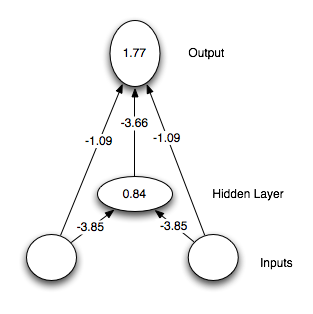
\includegraphics{xor.png}

\section{Encoding}

\subsection{Problem Statement}

The encoding problem is that given the same number of input and output elements but a lower number of hidden elements, with all information flowing through the hidden elements and no direct connections between input and output, can the system preserve the input signal to the output elements even though it propagates through a lower number of hidden elements?  This in a sense is a question of ``encoding'', since the pattern presented at the input layer must somehow be encoded in the hidden layer in order to be faithfully reproduced in the output layer.  

\subsection{Experimental Process}

The experimental process was to create a network containing four input elements and four output elements connected by two hidden elements, and then train it with a training set where every possible four-element input pattern is mapped to an identical output pattern.  Then this setup was repeated while varying a variety of parameters to see the effect of different initial conditions on the encoding process.  

\subsection{Results}

This learning process was a little more rocky than that for the XOR problem.  Given all 16 possible input patterns, a learning momentum of 0.4 and an epoch size of 128, the RMS error only ever reached a baseline of about 0.2004.  Many trials resulted in local minima where substandard results got locked in, giving a classification rate matrix deviating far from the desired diagonal matrix.  Changing the epoch size did not seem to affect the quality of the results.  

Increasing the learning momentum above a certain level (around 0.8) resulted in chaotic dynamics that never settled on any particular weights configuration.  Lowering the learning momentum only slowed the results, but did not result in any dramatic difference in the essential dynamics.  Here is the weights and biases from one of the more successful runs (this was after about 30000 runs):

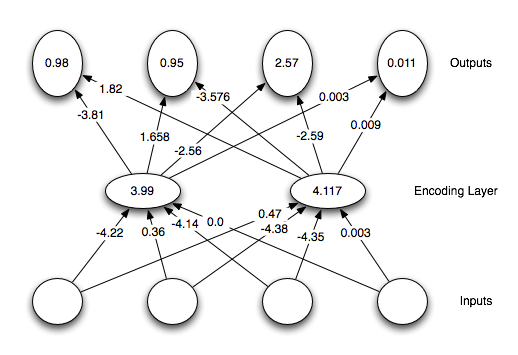
\includegraphics[scale=0.8]{encoding.png}

\end{document} 

